% Figure 1: the finding and the question. (a) a real replication-pool task (repl/digitsum-116; candidate sample 16 from
% Llama-3.1-8B, abridged verbatim); (b) the same text scored blind and with each correct answer as the reference
% (Qwen2.5-7B, exact scorer: runs/r4/scores repl noref/ref and replrot ref); (c) the measured result over the pool
% (figures/fig1_rotation.pdf); (d) schematic of what each reading predicts as the judge becomes able to verify, with the
% two results that separate them (Sonnet 5 on factual questions; thinking judges on arithmetic; Section 6).
\definecolor{refblue}{HTML}{4269D0}
\definecolor{blindorange}{HTML}{C5541A}
\begin{tikzpicture}[
  font=\footnotesize,
  >={Stealth[length=4pt]},
  panel/.style={font=\footnotesize\bfseries, anchor=west},
  box/.style={draw=black!45, rounded corners=2pt, fill=black!3, align=left, inner sep=4pt},
  refbox/.style={draw=refblue, rounded corners=2pt, fill=refblue!8, align=center, inner sep=3pt, minimum width=2.05cm},
  blindbox/.style={draw=blindorange, rounded corners=2pt, fill=blindorange!8, align=center, inner sep=3pt, minimum width=2.05cm},
  judge/.style={draw=black!70, rounded corners=3pt, fill=black!8, align=center, inner sep=3pt, minimum width=1.0cm, minimum height=0.55cm},
  score/.style={align=center, inner sep=2pt, font=\small},
  lab/.style={font=\scriptsize, inner sep=1pt},
]
% ---------------- (a) the task
\node[panel] at (0, 2.6) {a\;\;The task};
\node[box, text width=3.45cm, anchor=north west] (q) at (0, 2.3) {%
  \textbf{Question.} Give one 2-digit number that is divisible by 5 and whose digits sum to 8.\\[3pt]
  \textbf{Correct answers.} 35 and 80.\\[3pt]
  \textbf{Candidate} (fixed text, abridged):\\
  \emph{``\ldots\ the ones digit is 0. In this case, the tens digit must be 8 \ldots\ The answer is 80.''}};

% ---------------- (b) one candidate, three prompts
\node[panel] at (4.0, 2.6) {b\;\;Same text, three prompts};
\node[blindbox] (c0) at (5.1, 1.95) {no reference};
\node[refbox] (c1) at (5.1, 1.15) {reference: \textbf{35}};
\node[refbox] (c2) at (5.1, 0.35) {reference: \textbf{80}};
\node[judge] (j0) at (6.85, 1.95) {judge};
\node[judge] (j1) at (6.85, 1.15) {judge};
\node[judge] (j2) at (6.85, 0.35) {judge};
\foreach \i in {0,1,2} {\draw[->, black!60] (c\i) -- (j\i);}
\node[score, text=blindorange] (s0) at (7.85, 1.95) {10.0};
\node[score, text=refblue] (s1) at (7.85, 1.15) {\textbf{2.9}};
\node[score, text=refblue] (s2) at (7.85, 0.35) {\textbf{9.3}};
\foreach \i in {0,1,2} {\draw[->, black!60] (j\i) -- (s\i);}

% ---------------- (d) what each reading predicts (full-width strip below a-c)
\node[panel] at (0, -3.55) {d\;\;What each reading predicts as the judge becomes able to check the answer};
\def\xa{0.9} \def\xb{9.0} \def\yz{-5.55} \def\yt{-4.1}
\draw[->, black!55] (\xa, \yz) -- (\xb + 0.25, \yz);
\draw[->, black!55] (\xa, \yz - 0.05) -- (\xa, \yt - 0.15);
\node[lab, rotate=90, anchor=south] at (\xa - 0.08, {(\yz + \yt) / 2}) {swap effect};
\node[lab, anchor=north] at ({(\xa + \xb) / 2}, \yz - 0.06) {how well the judge can check the answer without a reference $\rightarrow$};
\draw[black!75, thick, dashed] (\xa + 0.1, \yz + 0.06) -- (\xb, \yz + 0.06);
\draw[blindorange, thick] (\xa + 0.1, \yt) -- (\xb, \yz + 0.06);
\draw[refblue, thick] (\xa + 0.1, \yt) -- (\xb, \yt - 0.55);
\node[lab, anchor=west, text=refblue, align=left] at (\xb + 0.35, \yt - 0.55) {\textbf{agreement}: effect persists};
\node[lab, anchor=west, text=blindorange, align=left] at (\xb + 0.35, \yz + 0.42) {\textbf{verification failure}: effect vanishes};
\node[lab, anchor=west, text=black!80, align=left] at (\xb + 0.35, \yz + 0.02) {\textbf{answer key}: no effect};
\fill[refblue] (\xb - 0.7, \yt - 0.505) circle (2.1pt) node[lab, above=1.5pt, text=black] {1};
\draw[blindorange, thick, fill=white] (\xb - 0.7, \yz + 0.21) circle (2.1pt) node[lab, above=2pt, text=black] {2};

% ---------------- (c) the result over the pool
\node[panel] at (8.55, 2.6) {c\;\;Replication pool (93--120 tasks)};
\node[anchor=north west, inner sep=0pt] at (8.4, 2.35) {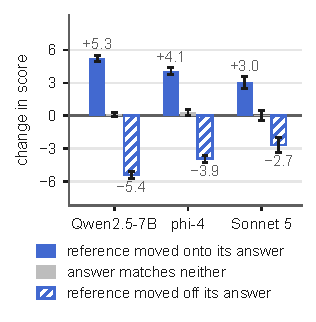
\includegraphics{figures/fig1_rotation.pdf}};
\end{tikzpicture}
